% Document class
\documentclass[10pt]{article}

% Preamble
\usepackage[a4paper,margin=2.5cm,includefoot]{geometry} % includefoot makes footer stay inside of the page
\usepackage{titling}
\usepackage{fancyhdr}
\usepackage[hidelinks]{hyperref}
\usepackage[czech]{babel}
\usepackage{amsthm}
\usepackage{mathtools}
\usepackage{enumitem} % for a,b,c enums
\usepackage{caption}

% FONT SPEC (for XeLaTeX) TO MAKE TROJA PRINTER WORK
\usepackage{fontspec}
\usepackage{unicode-math}

%% metadata settings
\newcommand{\tutnum}{0}
\title{\tutnum. cvičení z diskrétní matematiky}
\author{Jan Hartman}
\date{29.9.2025}

\newcommand{\teacherurl}{https://kam.mff.cuni.cz/~hartmaj/}
\newcommand{\titlerule}{%
    \noindent %
    \makebox[\textwidth]{\large \thetitle \hfill \thedate}
    \rule{\textwidth}{0.4pt}%
}

% remove default caption by czech babel
\captionsetup[figure]{labelformat=empty}

%% headers and footers settings
\renewcommand{\headrulewidth}{0pt}
\renewcommand{\footrulewidth}{0.4pt}
\pagestyle{fancy}
\fancyhf{} % clear all header/footer (e.g. by default, footer would show page numbers)
% \fancyhead[L]{\thetitle}   % left -> title
% \fancyhead[C]{} % center -> unused
% \fancyhead[R]{\thedate}  % right -> date
\fancyfoot[C]{\small Více info k cvičení: \url{\teacherurl}}  


% theorem styles
\newtheoremstyle{definitionstyle}{10pt}{10pt}{\normalfont}{}{\bfseries}{.}{ }{\thmname{#1}}
\newtheoremstyle{problemstyle}{10pt}{10pt}{\normalfont}{}{\bfseries}{.\newline}{ }{\thmname{#1}\thmnumber{ #2}\thmnote{ (#3)}}

% theorems
\theoremstyle{definitionstyle}
\newtheorem{defn}{Definice}
\theoremstyle{problemstyle}
\newtheorem{problem}{Příklad}

% Document body
\begin{document}

\titlerule

\section{Výroky}

\begin{minipage}{0.7\textwidth}
V následujících příkladech uvažujeme množinu států: $$M = \{ \text{Francie}, \text{Německo}, \text{Česko}, \text{Slovensko} \}$$ a nechť $V(x,y)$ je zkratka pro výrok: „Stát $x$ vyváží víno do státu $y$.“. Vztah $V$ je znázorněn na diagramu vpravo.
\end{minipage}%
\hfill
\begin{minipage}{0.15\textwidth}
  \centering
  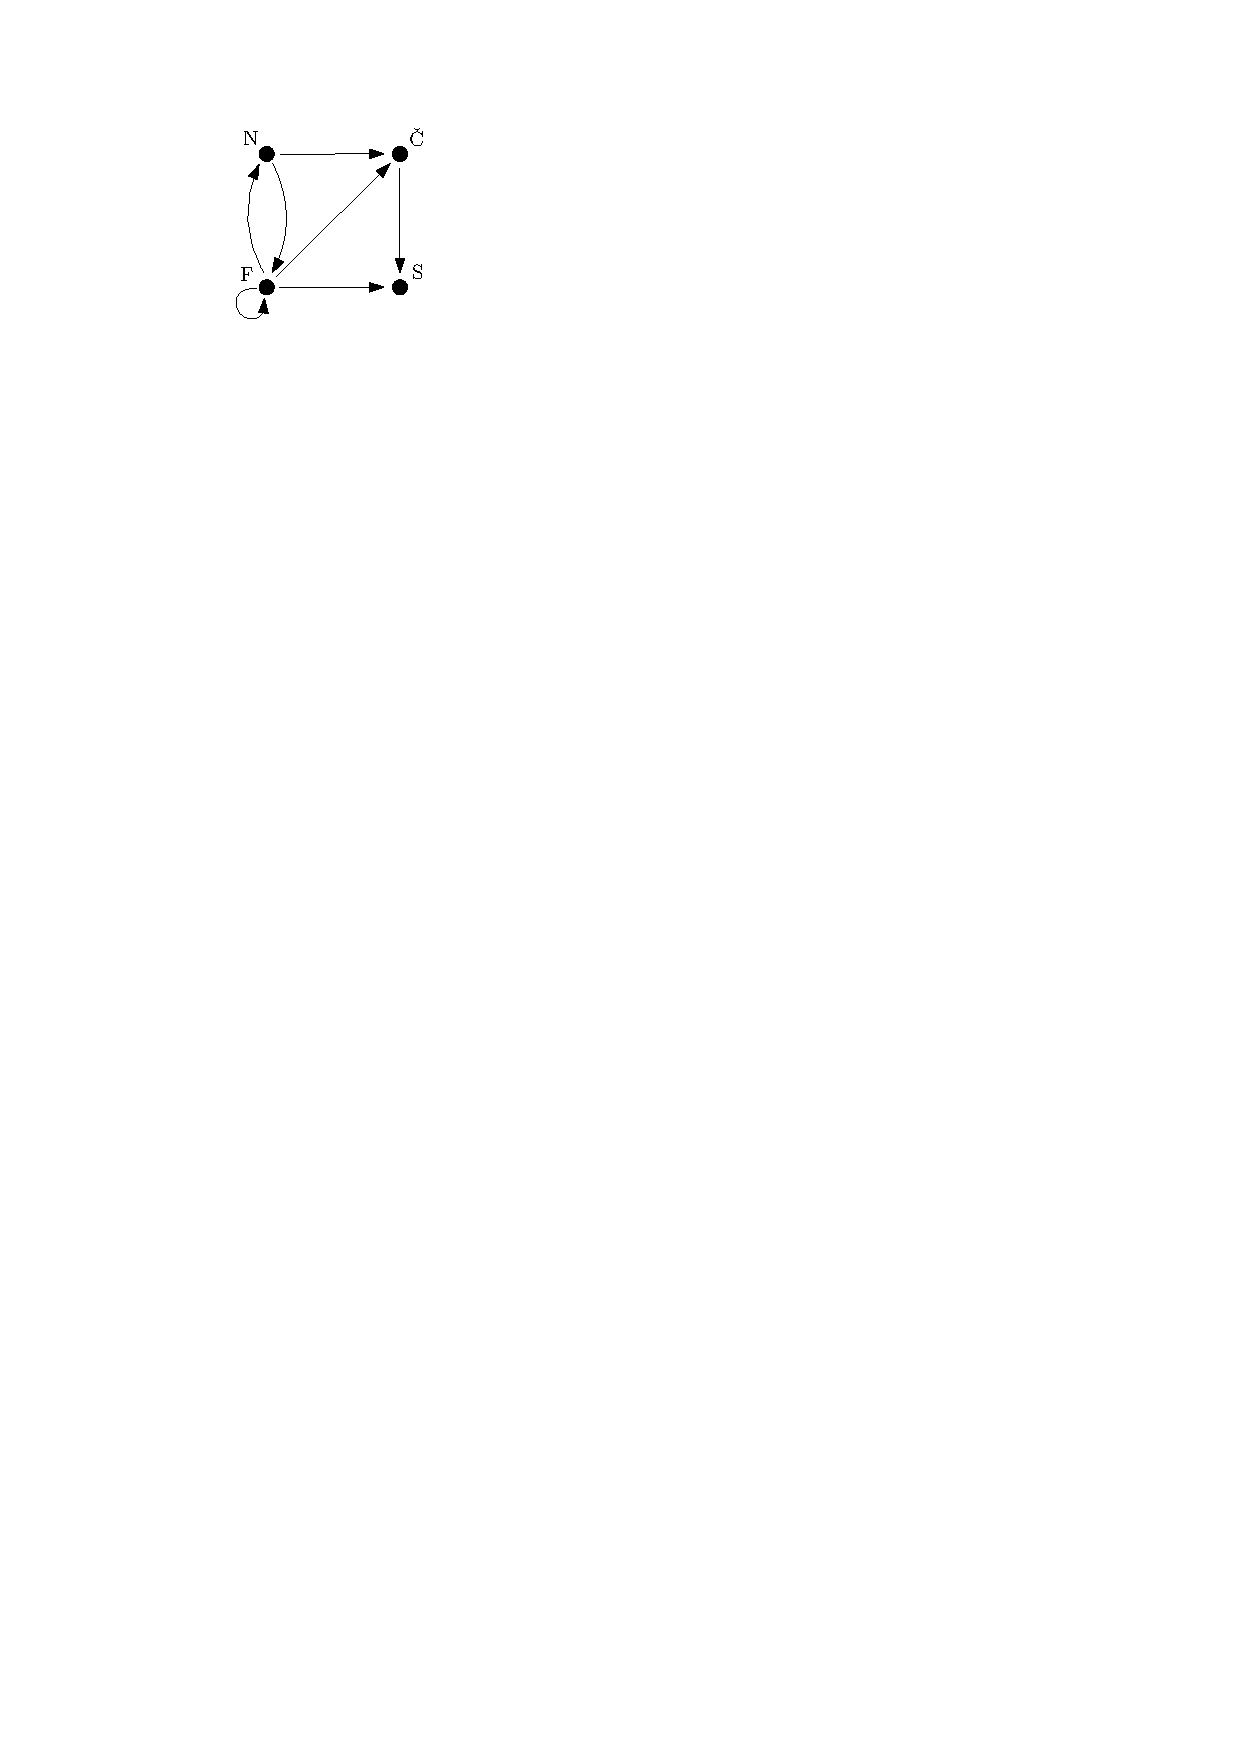
\includegraphics[width=2.2cm]{states.pdf}
\end{minipage}

\begin{problem}[Překládání]
Vyjádřete výroky v přirozeném jazyce matematickými symboly a naopak:
\begin{enumerate}[label=(\alph*)]
    \item \text{Slovensko vyváží víno do Francie.}
    \item $\exists y \in M : V(\text{Německo},y)$
\end{enumerate}
\end{problem}

\begin{problem}[Pořadí kvantifikátorů]
Vyjádřete následující výroky slovy a následně určete, zda jsou pravdivé či lživé:
\begin{enumerate}[label=(\alph*)]
    \item $\forall x \in M \ \exists y \in M : V(x,y)$
    \item $\forall x \in M \ \exists y \in M : V(y,x)$
    \item $\exists x \in M \ \forall y \in M : V(x,y)$
    \item $\exists x \in M \ \forall y \in M : V(y,x)$
\end{enumerate}

\end{problem}

\begin{problem}[Důkazy]
O jisté množině států $E$ jsme zjistili, že splňujě:
\begin{enumerate}
    \item $\forall x \in E \ \forall y \in E: V(x,y) \Rightarrow \neg V(y,x)$
    \item $\forall x \in E \ \forall y \in E \  \forall z \in E : V(x,y) \wedge V(y,z) \Rightarrow V(x,z)$
\end{enumerate} 
\begin{enumerate}[label=(\alph*)]
    \item Zkuste formulovat podmínky vlastními slovy. Splňuje tyto podmínky i množina $M$ zmíněná výše?
    \item Dokažte, že v $E$ neexistuje stát, který vyváží víno sám sobě.
    \item* Dokažte, že v $E$ neexistuje posloupnost států $x_0, \ldots , x_n$ t.ž. $V(x_0,x_1) \wedge V(x_1,x_2) \wedge \ldots \wedge  V(x_{n-1},x_n)$ kde $x_0 = x_n$.

\end{enumerate}

\end{problem}

\section{Množiny}

\begin{defn}
    Symetrický rozdíl $A \bigtriangleup B$ definujeme jako množinu prvků, které jsou buď v $A$, anebo v $B$ (ale ne v $A$ i $B$ zároveň).
\end{defn}

\begin{problem}[Symetrický rozdíl pomocí ostatních operací]
Zapište množinu $A \bigtriangleup B$ pomocí množinových operací $\cup, \cap, \setminus$. Nemusíte využít všechny uvedené operace. Zkuste najít aspoň dva způsoby.
\end{problem}

\begin{problem}[Dvouprvkové podmnožiny]
Mějme libovolnou množinu $K$. Uvažme všechny její podmnožiny obsahující právě dva prvky. Jaké množiny jsme z nich schopni vytvořit pomocí operace $\bigtriangleup$? Jsme takto schopni zkonstruovat libovolnou podmnožinu množiny $K$?
\end{problem}

\begin{problem}[Operace na množinách]
Určete maximální počet různých množin, které můžeme získat z množin $A,B$ aplikováním operací $\cup, \cap, \setminus$. Operace můžete opakovat i kombinovat. Stejně tak můžete libovolnou z množin použít vícekrát.
\end{problem}

\section{Hádanky}

\begin{problem}[Topinky]
Jakožto chudý student nemající dost peněz na topinkovač si smažíme topinky na pánvi. Opéci jednu stranu topinky trvá 5 minut. Na pánev se vejdou současně nejvýš dva krajíce. Jak dlouho bude trvat opečení 3 krajíců chleba? Jak dlouho bude trvat opéct $n$ krajíců chleba?
\end{problem}

\begin{problem}[Rovnoramenná váha]
Máme k dispozici rovnoramennou váhu a 9 mincí. Jedna z mincí je ovšem falešná, což se pozná tak, že je lehčí než ostatní mince, které váží všechny stejně. Na kolik nejméně vážení dokážeme zjistit, která z mincí je falešná?
\end{problem}

\begin{problem}[Hazard]
V casinu ti nabídli následující hru: Nejprve zaplatíš 1 euro za vstup do hry. Dále je před tebe položeno 6 přihrádek, kde v každé leží jeden cent. Můžeš ve kterémkoliv tahu vyjmout obsah všech přihrádek, takto získanou částku si ponechat a odejít ze hry. Dále můžeš zahodit jeden cent z nějaké přihrádky a vložit dva centy do přihrády bezprostředně napravo od ní.

\begin{enumerate}[label=(\alph*)]
\item Vyplatí se ti přijmout nabídku a hrát?
\item Máš k dispozici navíc akci: Zahodit cent z nějaké přihrádky a prohodit obsah dvou přihrádek bezprostředně vpravo od této přihrádky. Kolik peněz zvládneš vydělat nyní?
\end{enumerate}

\end{problem}

\vspace{1cm}

\begin{figure}[h]
    \centering
    
\includegraphics[width=12cm]{hazard_setup.pdf}
    \caption{Počáteční rozložení přihrádek}
\end{figure}

\vspace{1cm}

\begin{figure}[h]
    \centering
    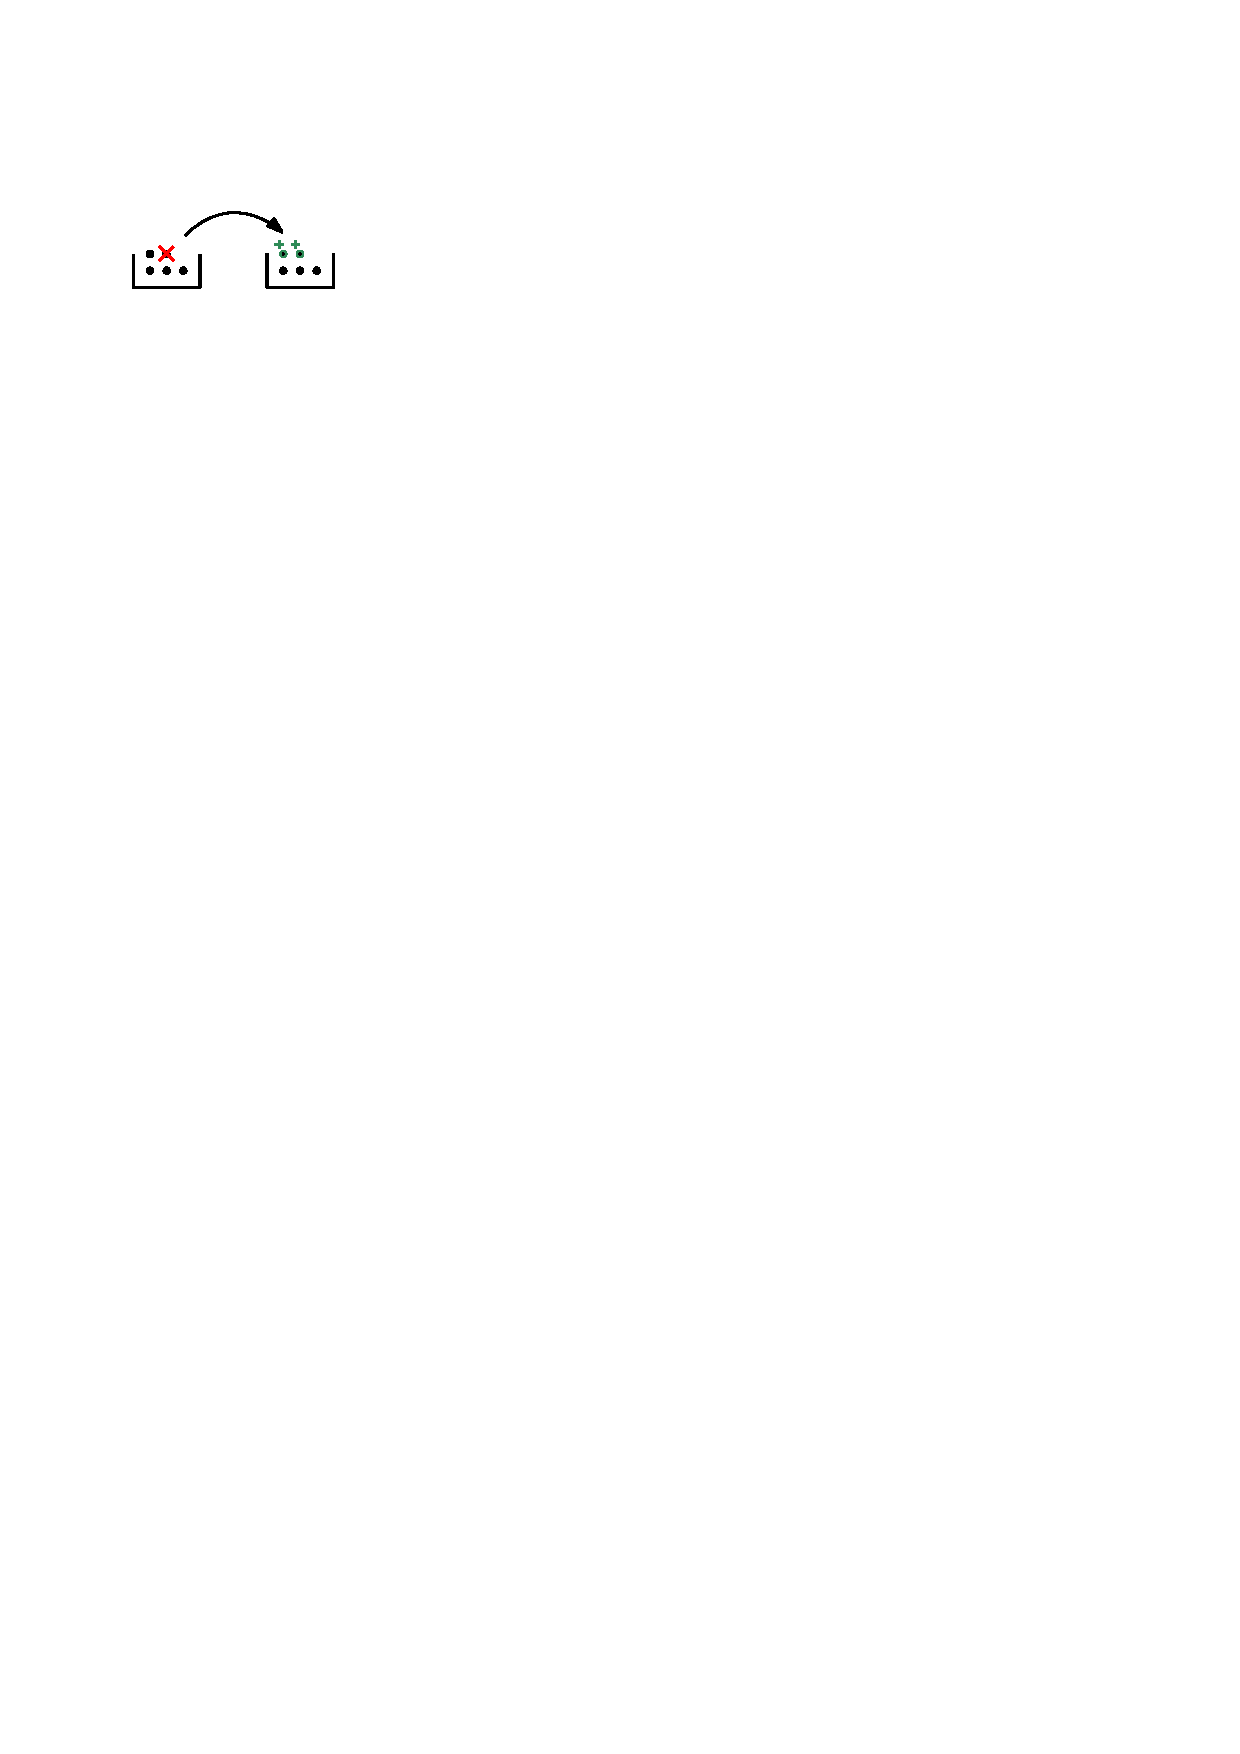
\includegraphics[width=4cm]{hazard_rule_1.pdf}
    \caption{Základní pravidlo}
\end{figure}

\vspace{1cm}

\begin{figure}[h]
    \centering
    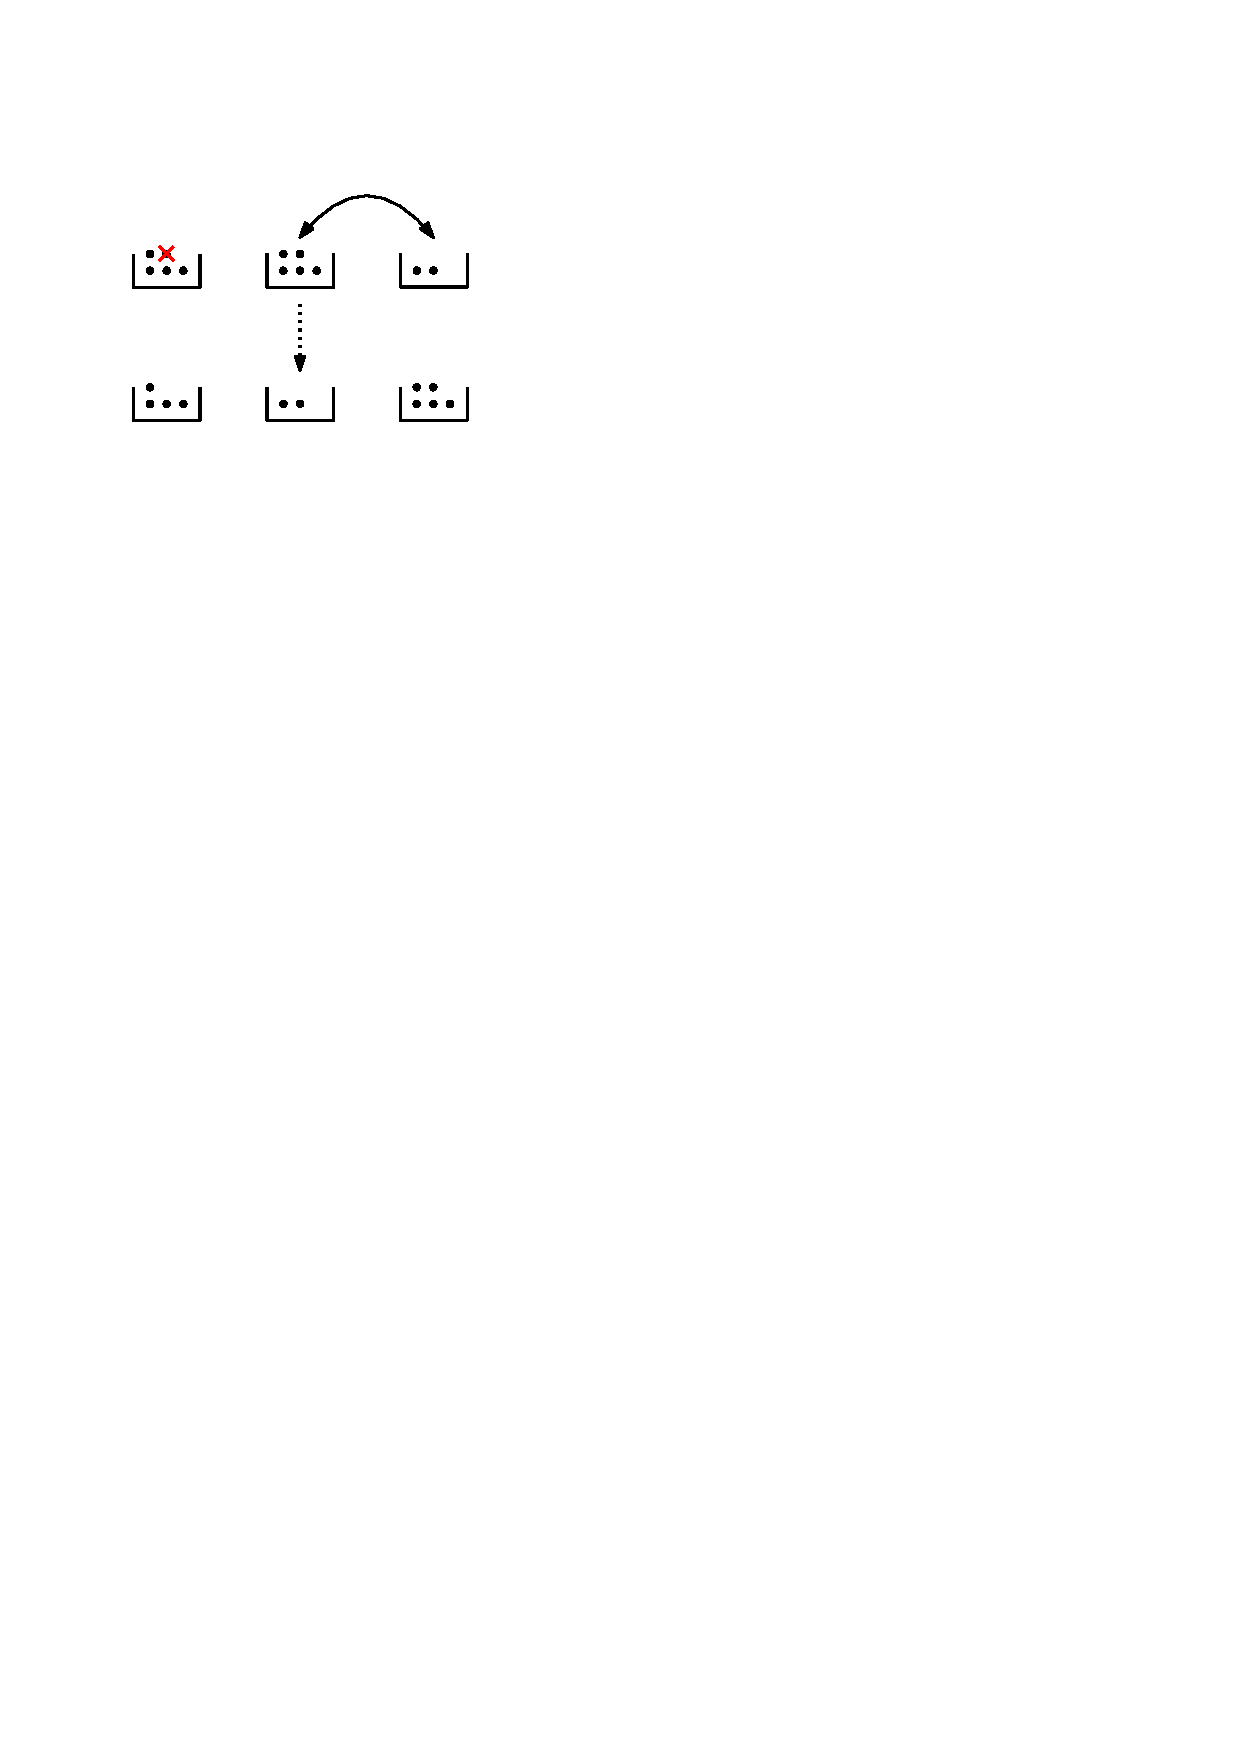
\includegraphics[width=6cm]{hazard_rule_2.pdf}
    \caption{Pravidlo navíc}
\end{figure}

\end{document}